\section{Use Cases and Numerical Experiments}
\label{chap:useCases}

In this section, we describe two use cases (Section~\ref{chap:CnR} and~\ref{chap:Netzfahrplan}) to which we are able to apply the methods mentioned before. For each use case we provide numerical experiments showing the threefold benefit of faster response times, increased capacity usage and reduced travel times.

\subsection{Click\&Ride App}
\label{chap:CnR}
For a short-term train path request, e.g.\ a train run for the next day, we can improve the response time to the railway operator by using our approach in a fully automated process. We will introduce the new way of booking a train path with a mobile application called \emph{Click\&Ride-App}. We commit to provide the railway operator with a train path offering in at most three minutes. In comparison, today's process for manual planning takes several hours in most cases and may require up to three days. To ensure a maximum duration of three minutes we need to automate every single step in the planning process. A simplified process sequence is shown in Figure~\ref{fig:process_sequence}.
%
\begin{figure}[htb]
	\centering
	% If you include a JPG file,
	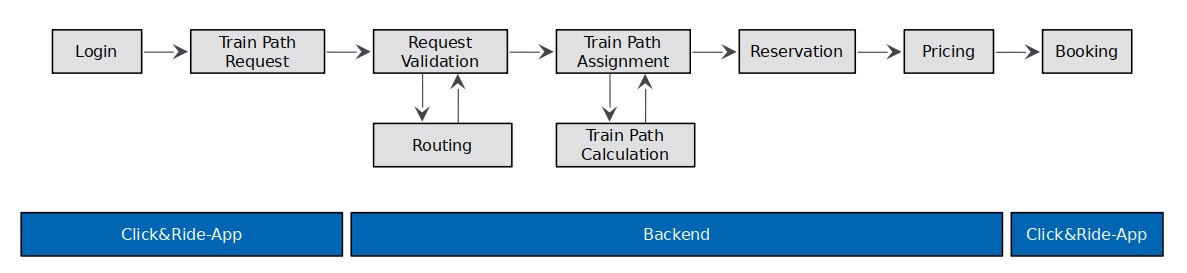
\includegraphics[width=\textwidth]{Bilder/process_sequence.jpg}
	% Else if you include an EPS file
	%    (it may need an interpreter for the PostScript language, e.g. Ghostscript),
	%\includegraphics[scale=0.30]{Fig1_Track.eps}
	\caption{Simplified process of Click\&Ride. The process is fully automated except for login and requesting a train path as well as booking.}
	\label{fig:process_sequence}
\end{figure}

Click\&Ride is a new B2B channel so only railway operators may use the functionalities. After logging in, the the train path request will be submitted to the back-end processes. At first there is a validation service that ensures formal and technical fit to the lines that will be used. For example an electric vehicle cannot use a track with no overhead line. If there are any problems with the train path request the railway operator gets instant feedback on the app's screen and can fix the problem. When there are no problems left the train path request is handled by the optimization in train path assignment (see Section~\ref{chap:Belegung}). If the technical properties of the requested train do not match the existing slots on the lines, a train path is generated automatically by train path planning as described in Section~\ref{chap:Konstruktion}. Railway operators have a limited time to check the offered train path before booking. To make sure the capacity on the line cannot be given to other railway operators in the meanwhile, the train path is reserved for a maximum of ten minutes. To complete the response the total price for the train path is calculated and displayed in the Click\&Ride-App. An example response is shown in Figure~\ref{fig:CnR_response}.
\begin{figure}[htb]
	\centering
	% If you include a JPG file,
	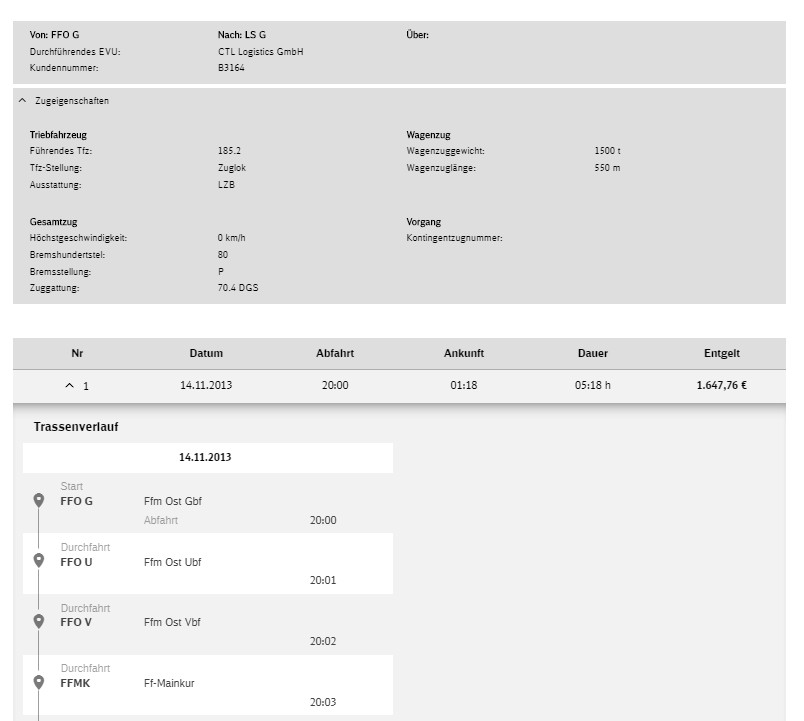
\includegraphics[width=\textwidth]{Bilder/train_path.jpg}
	% Else if you include an EPS file
	%    (it may need an interpreter for the PostScript language, e.g. Ghostscript),
	%\includegraphics[scale=0.30]{Fig1_Track.eps}
	\caption{Example Train Path in Click\&Ride}
	\label{fig:CnR_response}
\end{figure}

\subsubsection{Numerical Experiments}
For our experiments we use $1182$ real customer requests from November, 14th, 2013 in Germany. A customer request consists of the waypoints, time requirements and the characteristics of the train. The waypoints are at least the start of the request and its goal, but may also include some stops which should be served in between. The time requirements for our data consists only of an interval at the start of the request. But it is also possible to provide further time restrictions on the other waypoints. The characteristics of the request include all data necessary to calculate its dynamic properties such as acceleration and its static parameters like length, width and mass of the requested train. We consider the actual German infrastructure available in 2013. Furthermore, we also regard the blockages of passenger trains, which were scheduled on November, 14th, 2013 in order to have a realistic setup.
%
\begin{table}[h]
	\centering
	\caption{Response times in seconds for $1182$ requests provided in percentiles.}
	\label{tab:result_CnR}
	\begin{tabular}{ccccc} \hline
		$\textbf{50\%}$ & $\textbf{90\%}$ & $\textbf{95\%}$ & $\textbf{99\%}$ \\ \hline
		$8.47$ sec.     & $66.74$ sec.    & $138.30$ sec.   & $216.55$ sec.   \\
	\end{tabular}
\end{table}
\par

The experiments, as provided in Table~\ref{tab:result_CnR}, show that $95\%$ of the request are served within $138.30$ seconds and the maximal response time is $431.10$ seconds. This is a vast improvement compared to the up to three days required in the current manual process. We plan to improve response times further in order to comply with our three minute target even in the $99$ percentile.
\textbf{\textcolor{red}{ADD INTERNAL BFQ plus die Erklärung BFQ, da es hier zum ersten Mal auftritt.}}

\subsection{Annual Timetable}
\label{chap:Netzfahrplan}

The introduced methods will allow us to change the process of the creation of an annual timetable. In this use case all customer requests, for passenger and freight trains, are put at the same time and have to be provided with a timetable fulfilling all requests within $50$ days. This currently means a huge effort to DB Netz and can be eased by planning the freigth trains automatically. In an iterative process we manually create timetables for the passenger trains first. In the second step, the freight trains are calculated automatically with the methods described in Sections~\ref{chap:Konstruktion} and~\ref{chap:Belegung}. Afterwards the timetables are adapted and improved iteratively.

\begin{figure}[htb]
	\centering
	% If you include a JPG file,
	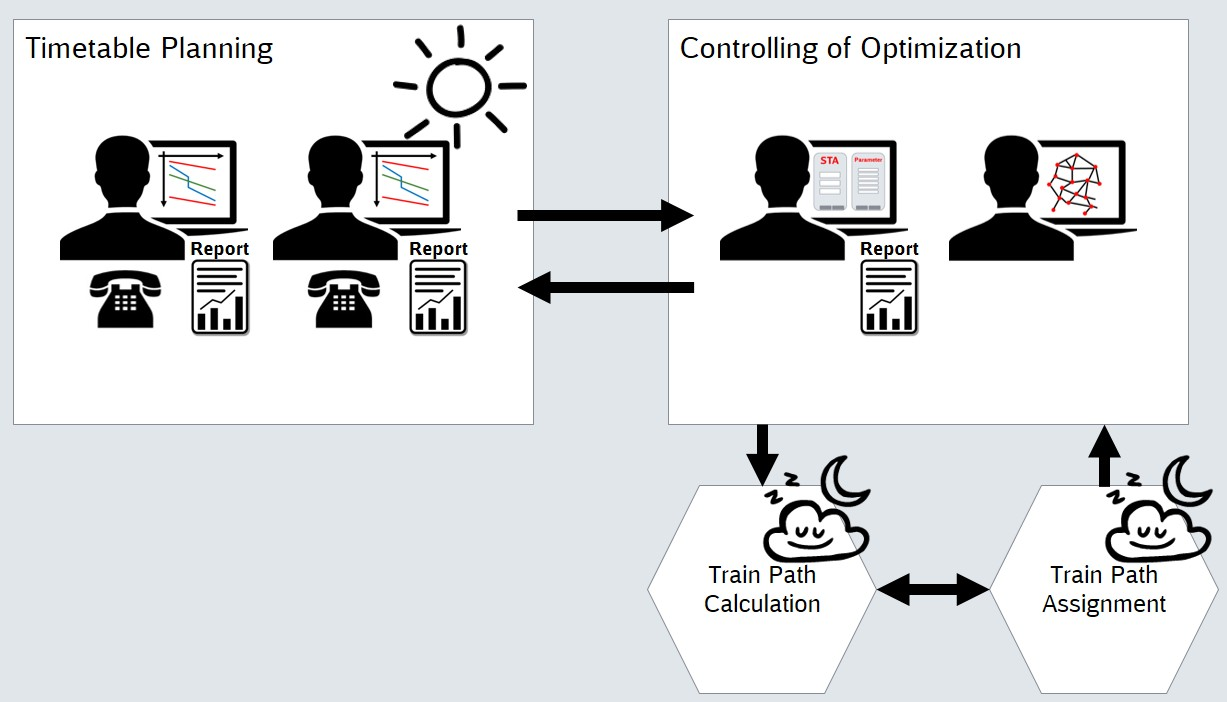
\includegraphics[width=\textwidth]{Bilder/annual_planning.jpg}
	% Else if you include an EPS file
	%    (it may need an interpreter for the PostScript language, e.g. Ghostscript),
	%\includegraphics[scale=0.30]{Fig1_Track.eps}
	\caption{Iterative Process for Annual Timetable: Planning by hand during the day and automated optimization during the night}
	\label{fig:annual_planning}
\end{figure}

\subsubsection{Numerical Experiments}
For this experiment we again consider the data from November, 14th, 2013 regarding infrastructure, blockages and customer requests. For clarity of presentation we restrict the shown results to the German part of Corridor One (the Rhine-Alpine Corridor) \cite{} rather than the entire German network. Corridor One stretches from sea ports of Rotterdam, Zeebrugge, Antwerp, Amsterdam and Vlissingen to the port of Genoa. It covers five different countries: Netherlands, Belgium, Germany, Switzerland and Italy. Here only the part in Germany from Emmerich and Aachen to Basel will be considered. (see picture \textbf{\textcolor{red}{XXX}}). We have a test set consisting of 210 requests and create 935,814 slots on 38 sections (compare \textbf{\textcolor{red}{Figure~\ref{}}}).
As before a customer request consists of the waypoints, time requirements and the characteristics of the train.


\begin{table}[h]
	\centering
	\caption{Results for the creation of slots}
	\label{tab:result_Netzfpl}
	\begin{tabular}{lcccc} \hline
		\textbf{KPIs Konstruktion}   & \textbf{Result}  \\ \hline
		Number of slots             & $935\,814$                      \\
		computing time       & 02:25h                     \\
		percentage rise Langerwehe (KLAW)   & $98.30\%$                       \\
		percentage rise Bensheim (FBH) & $102.83\%$                       \\
		percentage rise Oberwesel (FOBW) & $106.82\%$                     \\ \hline
	\end{tabular}
\end{table}
\par

\begin{table}[h]
	\centering
	\caption{Results for the train path assignment}
	\label{tab:result_Netzfpl_Bel}
	\begin{tabular}{lcccc} \hline
		\textbf{KPIs Belegung}   & \textbf{Result}  \\ \hline
		Number of Customer Requests             & $210$                      \\
		computing time       & 02:57h                     \\
		percentage train path assignments on slots   & $80\%$                       \\
		average BFQ & $1.27\%$                             \\ \hline
	\end{tabular}
\end{table}
\par

The experiments, as provided in Table \ref{tab:result_Netzfpl} and \ref{tab:result_Netzfpl_Bel}, show that the creation of the timetable for Corridor One takes about $5.5$ hours to assign $210$ customers' request on $935\,814$ slots, where $80\%$ of the requests use the systemized slots and the average BFQ of them is $1.27\%$. This is also a vast improvement compared to serveral days currently required in the manual process. Moreover it shows that the way we produce our slots is more efficient than the manual ones, since we are able to utilize more capacity on the infrastructure. This can be seen by the percentage rise of different points, e.g. Bensheim, where we produce $2.83\%$ more slots then we did manual in 2013 \textbf{\textcolor{red}{More explanation needed}}.